% -*- mode: latex; -*- mustache tags:  
\documentclass[10pt,twoside,english]{_support/latex/sbabook/sbabook}
\let\wholebook=\relax

\usepackage{import}
\subimport{_support/latex/}{common.tex}

%=================================================================
% Debug packages for page layout and overfull lines
% Remove the showtrims document option before printing
\ifshowtrims
  \usepackage{showframe}
  \usepackage[color=magenta,width=5mm]{_support/latex/overcolored}
\fi


% =================================================================
\title{Learning Object-Oriented Programming, Design and TDD with Pharo}
\author{Stéphane Ducasse}
\series{The Pharo TextBook Collection}

\hypersetup{
  pdftitle = {Learning Object-Oriented Programming, Design and TDD with Pharo},
  pdfauthor = {Stéphane Ducasse},
  pdfkeywords = {Introduction, programming, design, testing, Pharo, Smalltalk}
}


% =================================================================
\begin{document}

% Title page and colophon on verso
\maketitle
\pagestyle{titlingpage}
\thispagestyle{titlingpage} % \pagestyle does not work on the first one…

\cleartoverso
{\small

  Copyright 2017 by Stéphane Ducasse.

  The contents of this book are protected under the Creative Commons
  Attribution-ShareAlike 3.0 Unported license.

  You are \textbf{free}:
  \begin{itemize}
  \item to \textbf{Share}: to copy, distribute and transmit the work,
  \item to \textbf{Remix}: to adapt the work,
  \end{itemize}

  Under the following conditions:
  \begin{description}
  \item[Attribution.] You must attribute the work in the manner specified by the
    author or licensor (but not in any way that suggests that they endorse you
    or your use of the work).
  \item[Share Alike.] If you alter, transform, or build upon this work, you may
    distribute the resulting work only under the same, similar or a compatible
    license.
  \end{description}

  For any reuse or distribution, you must make clear to others the
  license terms of this work. The best way to do this is with a link to
  this web page: \\
  \url{http://creativecommons.org/licenses/by-sa/3.0/}

  Any of the above conditions can be waived if you get permission from
  the copyright holder. Nothing in this license impairs or restricts the
  author's moral rights.

  \begin{center}
    
\includegraphics[width=0.2\textwidth]{_support/latex/sbabook/CreativeCommons-BY-SA.pdf}
  \end{center}

  Your fair dealing and other rights are in no way affected by the
  above. This is a human-readable summary of the Legal Code (the full
  license): \\
  \url{http://creativecommons.org/licenses/by-sa/3.0/legalcode}

  \vfill

  % Publication info would go here (publisher, ISBN, cover design…)
  Layout and typography based on the \textcode{sbabook} \LaTeX{} class by Damien
  Pollet.
}


\frontmatter
\pagestyle{plain}

\tableofcontents*
\clearpage\listoffigures

\mainmatter

\chapter{Sending a message is making a choice}\label{cha:messages}
In this chapter we explore an \textit{essential} point of object-oriented programming: Sending a message is making a choice! 

Object-oriented programming books often present \textit{late binding}: the fact that the method to execute will only be determined at runtime based on the receiver. In fact sending a message uses late binding to select the correct method. I like to use the term \textit{sending a message} because it stresses that simple
actions, such as sending a message, are also a powerful feature when used well. 

This aspect is often not really well put in perspective in teaching materials. Lectures often focus on inheritance but understanding the power of message passing it crucial to build good design.
This point is so central for me that this is the first point that I explain when I start lectures on advanced design to people already understanding object-oriented programming. In addition, most of
the Design Patterns are based on the fact that sending a message is actually selecting the correct method
based on the message receiver.

To illustrate how sending a message performs a dynamic choice, I will start taking a simple example available in the core of Pharo: the Booleans. Pharo defines Booleans as two objects: \textcode{true} and \textcode{false}. They are so fundamental that you cannot change their value. 
Still their implementation also use late binding in a really elegant way. 
 I will explain how the Boolean negation and the disjunction (or) are implemented. Then I will step back and analyse the forces in presence and their importance. 
\section{Negation: the not message}
Boolean negation has nothing special in Pharo: negating a boolean returned the negated value! 
For example the snippets below show this conventional behavior and vice versa.

Sending the message \textcode{not} to the Boolean \textcode{true} returns the Boolean \textcode{false}. 

\begin{displaycode}{plain}
true not
>>> false
\end{displaycode}

\begin{displaycode}{plain}
false not
>>> true
\end{displaycode}

Nothing fancy. Of course the message \textcode{not} can be sent to Boolean expressions (i.e. expressions whose execution return Booleans) as shown below:

\begin{displaycode}{plain}
(2 * 4 > 3) not
>>> false
\end{displaycode}

\begin{displaycode}{plain}
(#(1 2 3) includes: 5) not
>>> true
\end{displaycode}

Now while Pharo follows traditional Boolean logic, what is less traditional is the implementation of the way the computation is done to answer the correct value.
\section{Implementing not}
Take a couple of minutes and a piece of paper and think about the way you would implement this message. Try really to write the code for real.
\subsection{A first hint. }
A first hint that I can give you is that the solution (used in Pharo and that we want to study) does not use explicit conditional such as \textcode{ifTrue:} or \textcode{ifTrue:ifFalse:}.

Take a bit more time to think how you can implement not. 
What we can tell you is the solution is not based on bit fiddling and logical operation on small integers. The solution we are looking for is simple and elegant.
\subsection{A second hint.}
The second hint is that \textcode{true} and \textcode{false} are instances of different classes. \textcode{true} is (the unique) instance of the class \textcode{True} while \textcode{false} is (the unique) instance of the class \textcode{False}. Note the uppercase on class names. This situation is depicted in Figure \ref{figTrueFalseOnly}.

What you should see is that the fact that the solution has two different classes opens the door to have two different \textcode{not} implementations as shown by Figure \ref{figTrueFalseOnlySelectors}. Indeed, as we mention in early chapters, we can have one message and multiple methods that we will be selected and executed depending on the receiver of the message. 

Now you should be ready to get the solution. We should have a definition for the \textcode{true} defined in the class \textcode{True} and one for \textcode{false} in the class \textcode{False}.


\begin{figure}

\begin{center}
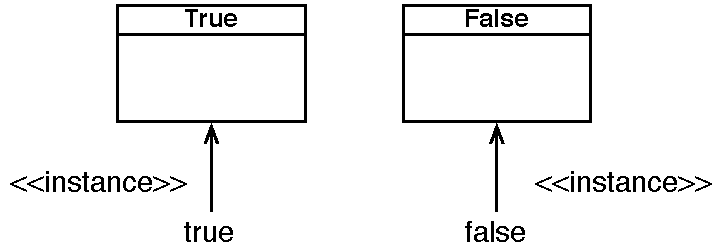
\includegraphics[width=0.55\textwidth]{/Users/ducasse/Workspace/FirstCircle/MyBooks/Bk-Writing/PharoBooks/LearningOOPWithPharoTrans/_result/pdf/Chapters/MessageSending/figures/BooleanTrueAndFalseSolelyWithInstances.pdf}\caption{The two classes \textcode{True} and \textcode{False} and their respective unique instances \textcode{true} and \textcode{false}.\label{figTrueFalseOnly}}\end{center}
\end{figure}



\begin{figure}

\begin{center}
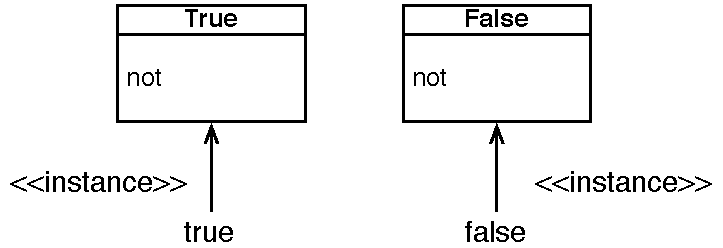
\includegraphics[width=0.65\textwidth]{/Users/ducasse/Workspace/FirstCircle/MyBooks/Bk-Writing/PharoBooks/LearningOOPWithPharoTrans/_result/pdf/Chapters/MessageSending/figures/BooleanTrueAndFalseWithNotMethodSelectors.pdf}\caption{Two methods for one message.\label{figTrueFalseOnlySelectors}}\end{center}
\end{figure}

\subsection{Studying the implementation}

\begin{figure}

\begin{center}
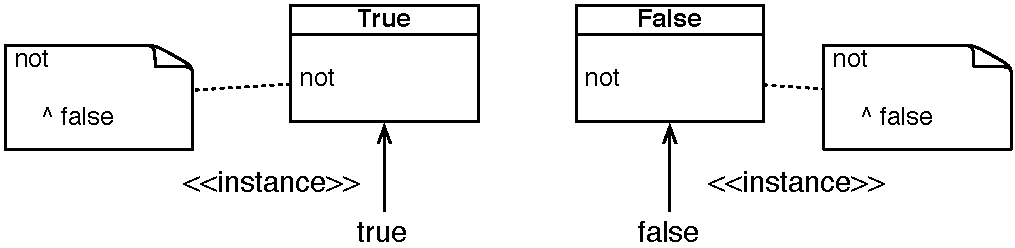
\includegraphics[width=0.75\textwidth]{/Users/ducasse/Workspace/FirstCircle/MyBooks/Bk-Writing/PharoBooks/LearningOOPWithPharoTrans/_result/pdf/Chapters/MessageSending/figures/BooleanTrueAndFalseWithNotMethods.pdf}\caption{Two methods for one message each one returning the other instance.\label{figTrueFalseSolution}}\end{center}
\end{figure}


The implementation of negation (message \textcode{not}) is defined as illustrated in Figure \ref{figTrueFalseSolution} and is shown below. The method \textcode{not} of the class \textcode{True} simply returns the Boolean \textcode{false}. 

\begin{displaycode}{plain}
True >> not
   "Negation--answer false since the receiver is true."
   ^ false
\end{displaycode}

\begin{displaycode}{plain}
False >> not
   "Negation--answer true since the receiver is false."
   ^ true
\end{displaycode}

Figure \ref{figTrueFalseSolutionLookup} shows that sending a message to one of the two Booleans selects the method in the corresponding class. What is important to see is that when a method is executed the receiver is from the class (or subclass we will see that later) that defines the method. We can also say that when we define a method in a given class we know that the receiver is from this class. Obvious, isn't it! But important. The implementation can then use this information as an execution context. This is exactly what the \textcode{not} implementation does. The method \textcode{not} defined on the class \textcode{True} knows that the receiver is true so it just has to return \textcode{false}. 


\begin{figure}

\begin{center}
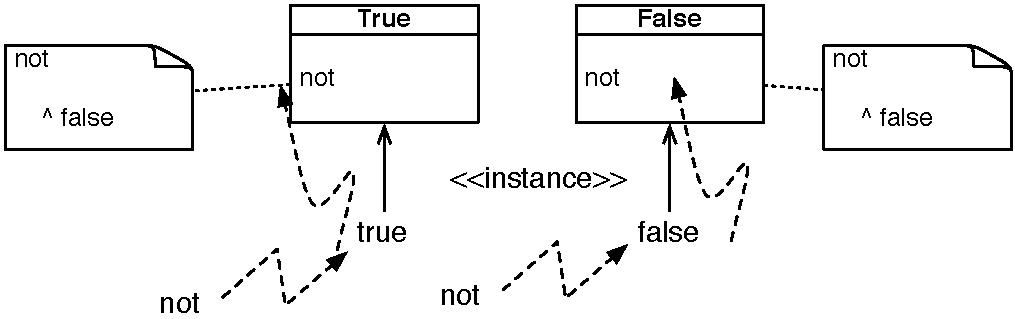
\includegraphics[width=0.75\textwidth]{/Users/ducasse/Workspace/FirstCircle/MyBooks/Bk-Writing/PharoBooks/LearningOOPWithPharoTrans/_result/pdf/Chapters/MessageSending/figures/BooleanTrueAndFalseWithNotMethodsLookup.pdf}\caption{Sending a message selects the method in the class of the receiver.\label{figTrueFalseSolutionLookup}}\end{center}
\end{figure}


\begin{note}
When we define a method in a given class we know that the receiver is from this class. Obvious but important. The implementation can then use this information.
\end{note}

Now we will see if you get it... Let us try with a slightly more complex example.
\section{Implementing disjunction}
Disjunction is also a core functionality of any programming language. In Pharo disjunction is expressed via the message \textcode{\textbar{}}. 
 Here are the traditional tables describing disjunction but expressed in Pharo: first starting with \textcode{true} as receiver.

\begin{tabular}{llll}
\toprule
\textbf{or} & true & false &  \\
true & true & true &  \\
false & true & false &  \\
\bottomrule
\end{tabular}

Here are a couple of examples expressed in Pharo. 

\begin{displaycode}{plain}
true | true
>>> true
\end{displaycode}

\begin{displaycode}{plain}
true | false 
>>> true
\end{displaycode}

\begin{displaycode}{plain}
false | false 
>>> false
\end{displaycode}

For the record, in fact the message \textcode{\textbar{}} implements an eager disjunction since it asks the value of its argument even when not needed and Pharo also offers lazy disjunction implemented in the message \textcode{or:} which only requests the argument value if needed.
\subsection{When receiver is true.}
Propose an implementation of the disjunction for the first case: i.e. when the receiver is the object \textcode{true}.

\begin{tabular}{llll}
\toprule
\textbf{or} & true & false &  \\
true & true & true &  \\
\bottomrule
\end{tabular}

 What you should have learned from the implementation of \textcode{not} is that you have two different methods taking advantage of the fact that they know what is the receiver during their execution. 

\begin{displaycode}{plain}
true | true 
>>> true
\end{displaycode}

\begin{displaycode}{plain}
true | false 
>>> true
\end{displaycode}

\begin{displaycode}{plain}
true | anything 
>>> true
\end{displaycode}

When you look at the table we see that when the receiver is \textcode{true} the result is the same as the receiver (i.e. \textcode{true}). In Pharo the method \textcode{\textbar{}} on class \textcode{True} express this as follows: 

\begin{displaycode}{plain}
True >> | aBoolean
   "Evaluating Or -- answer true since the receiver is true."
   ^ true
\end{displaycode}
\subsection{When receiver is false.}
Similarly let us study the Boolean table relative to false as receiver. 

\begin{tabular}{llll}
\toprule
\textbf{or} & true & false &  \\
false & true & false &  \\
\bottomrule
\end{tabular}

Here are some snippets

\begin{displaycode}{plain}
false | true 
>>> true
\end{displaycode}

\begin{displaycode}{plain}
false | false 
>>> false
\end{displaycode}

\begin{displaycode}{plain}
false | anything 
>>> anything
\end{displaycode}

We see that when the receiver is \textcode{false}, the result of the disjunction is the other argument. In Pharo the method \textcode{\textbar{}} on class \textcode{False} is then as follows: 

\begin{displaycode}{plain}
False >> | aBoolean
   "Evaluating Or -- answer with the argument, aBoolean."
   ^ aBoolean
\end{displaycode}


\begin{figure}

\begin{center}
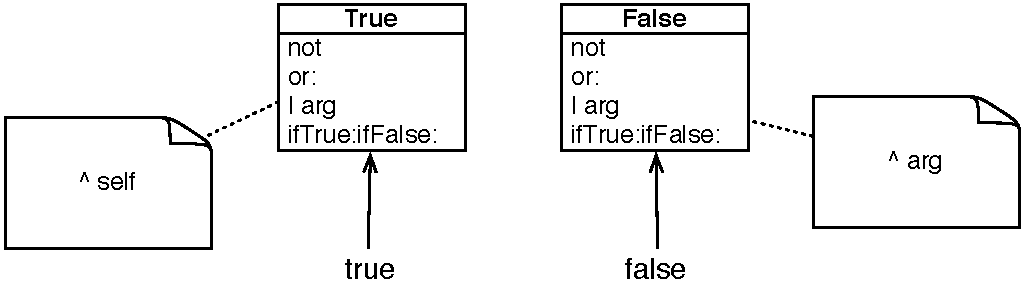
\includegraphics[width=0.8\textwidth]{/Users/ducasse/Workspace/FirstCircle/MyBooks/Bk-Writing/PharoBooks/LearningOOPWithPharoTrans/_result/pdf/Chapters/MessageSending/figures/BooleanNoHiearchyAndInstancesWithOrMethods.pdf}\caption{Disjunction implementation: two methods.\label{/Users/ducasse/Workspace/FirstCircle/MyBooks/Bk-Writing/PharoBooks/LearningOOPWithPharoTrans/_result/pdf/Chapters/MessageSending/figures/BooleanNoHiearchyAndInstancesWithOrMethods.pdf}}\end{center}
\end{figure}

\section{About ifTrue:ifFalse: implementation}
Now you should start to get the principle. Let us see how it works to also express conditional messages such as \textcode{ifTrue:ifFalse:}. Yes fundamental messages such as conditionals can be expressed using the same mechanism: late binding.

What you see with the following snippet is that message \textcode{ifTrue:ifFalse:} is expecting two different blocks as argument. 

\begin{displaycode}{plain}
4 factorial > 20
	ifTrue: [ 'bigger' ]
	ifFalse: [ 'smaller' ]
>>> 'bigger'
\end{displaycode}

Now you should know that to execute a block you should use the message \textcode{value} as illustrated:

\begin{displaycode}{plain}
[1 + 3] value
>>> 4
\end{displaycode}

Block can contain any expressions. The execution of the following block will open the Pharo logo.

\begin{displaycode}{plain}
[ (ZnEasy getPng: 'http://pharo.org/web/files/pharo.png')
       asMorph openInWindow ] value
\end{displaycode}

Let us come back to the case of condition and in particular to the message \textcode{ifTrue:ifFalse:}.
Based on the receiver we should execute the corresponding block from the \textcode{ifTrue:ifFalse:} method. When the expression (\textcode{4 factorial \textgreater{} 20} in the example above) is true we should execute the \textcode{ifTrue:} argument, when it is false we should execute the \textcode{ifFalse:} argument. 
\subsection{Implementation. }
The implementations is then simple and elegant.  In the \textcode{True} class, we want to execute the corresponding block, 
the one passed as \textcode{ifTrue:} argument as shown in Figure \ref{figFT}. 

\begin{displaycode}{plain}
True >> ifTrue: trueAlternativeBlock ifFalse: falseAlternativeBlock
   ^ trueAlternativeBlock value
\end{displaycode}

Similarly in the \textcode{False} class, we want to execute the corresponding block, 
the one passed as \textcode{ifFalse:} argument. 

\begin{displaycode}{plain}
False >> ifTrue: trueAlternativeBlock ifFalse: falseAlternativeBlock
   ^ falseAlternativeBlock value
\end{displaycode}


\begin{figure}

\begin{center}
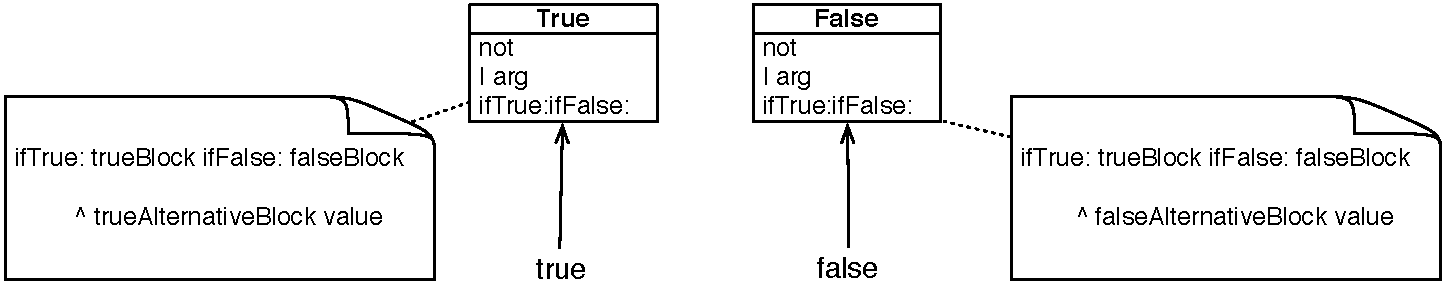
\includegraphics[width=1.0\textwidth]{/Users/ducasse/Workspace/FirstCircle/MyBooks/Bk-Writing/PharoBooks/LearningOOPWithPharoTrans/_result/pdf/Chapters/MessageSending/figures/BooleanNoHiearchyIFTMethods.pdf}\caption{Conditional implementation: again two methods and no explicit tests.\label{figFT}}\end{center}
\end{figure}

\subsection{Optimisation. }
What we show above works! But if you modify it, the modification will not be taken into account. 
This is because in Pharo \textcode{ifTrue:ifFalse:} is used so often and its semantics should not change that the compiler in fact does not send a message but convert it in low-level logic for the virtual machine. 
Now you can invent your own conditional message \textcode{siVrai:siFaux:} for a french version for example and you will see that this implementation works.
\section{What is the point?}
Some readers may be intrigued and think that this is spurious because they will never have to reimplement Booleans in their life. This is true even if there are different versions of Boolean logic such as the ternary logic that contains also unknown value. 

We picked the Boolean examples to illustrate an important point: sending a message is making a choice. The runtime system will dynamically select the method depending on the receiver. This is what is called late binding or dynamic dispatch. Only at execution the correct method is selected. Now the Boolean example is the simplest one I could find to illustrate this point. 
It is also ground breaking in the sense that it touches something as fundamental as Boolean main operations. 

Now the choices can be made over several dozens of classes. For example in Pillar the document processing system in which this book is written there are around 59 different classes expressing different parts of a document: section, title, bold, paragraph... and the same principle applies there. The system selects the correct methods to render text, LaTeX or HTML using exactly the same principle. 

Now most of the time you can express the same using conditions (except for the Boolean example and this is why I asked you to implement Boolean logic since you do not want to have Boolean logic to be based on condition because this is inefficient) as follows:

\begin{displaycode}{plain}
emitHTML: stream
	self == PRList
		ifTrue: [ ... ]
		self == PRParagraph 
			ifTrue: [ ... ]
			...
\end{displaycode}

The problems with such explicit conditions is the following: 

\begin{itemize}
\item First, they are cumbersome to write. Even using case statements as in other languages, the logic can become complex. Imagine for 59 cases of Pillar. Here is a small part of the document hierarchy. 
\end{itemize}

\begin{displaycode}{plain}
PRObject #(''properties'')
        PRDocumentItem #(''counter'')
                PRDocumentGroup #(''children'')
                        PRDocument #()
                        PRHeader #(''level'')
                        PRList #()
                                PROrderedList #()
                                PRUnorderedList #()
                        PRParagraph #()
                        PRReference #(''reference'' ''parameters'')
                                PRFigure #()
                        PRSlide #(''title'' ''label'')
                PRText #(''text'')'
\end{displaycode}

\begin{itemize}
\item Second, such definitions are not modular. It means that adding a new case requires to edit the method and recompile it. While with the dynamic dispatch, we can just add a new class as shown in Figure \ref{figFat}. Furthermore this class can just take advantage of an existing one and extend it (as we will explained in Chapter \ref{cha:inheritance}).
\end{itemize}


\begin{figure}

\begin{center}
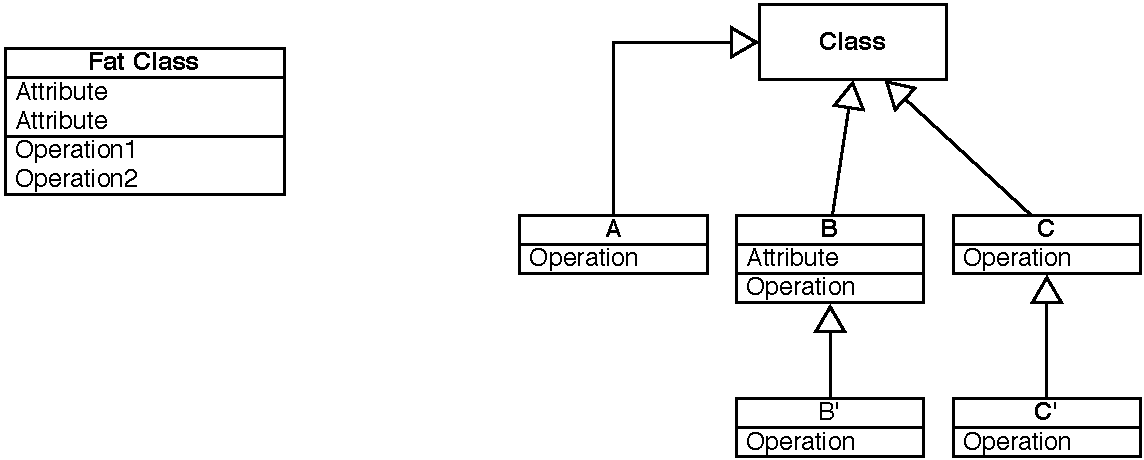
\includegraphics[width=0.8\textwidth]{/Users/ducasse/Workspace/FirstCircle/MyBooks/Bk-Writing/PharoBooks/LearningOOPWithPharoTrans/_result/pdf/Chapters/MessageSending/figures/Design-FatVsDispatch.pdf}\caption{One single class vs. a nice hierarchy.\label{figFat}}\end{center}
\end{figure}


You could think that this is a not a problem but imagine that now for a business you want to ship different products or solutions to your clients. With dynamic dispatch you can simply package alternate code in separate packages and load them independently as shown in Figure \ref{inhNoFatPackage}.


\begin{figure}

\begin{center}
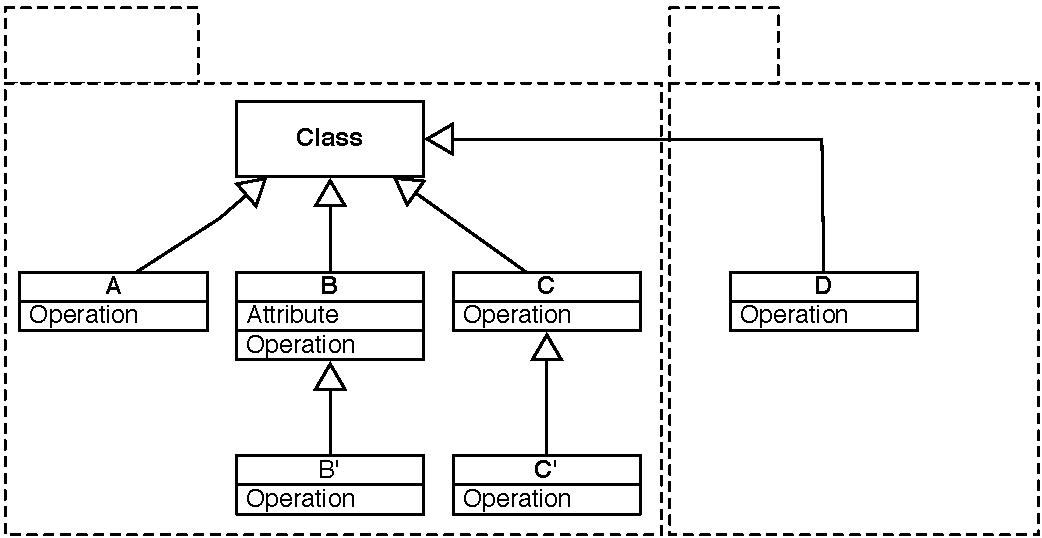
\includegraphics[width=0.8\textwidth]{/Users/ducasse/Workspace/FirstCircle/MyBooks/Bk-Writing/PharoBooks/LearningOOPWithPharoTrans/_result/pdf/Chapters/MessageSending/figures/Design-FatVsDispatchWithPackages.pdf}\caption{One single class vs. a nice hierarchy.\label{inhNoFatPackage}}\end{center}
\end{figure}

\subsection{Classes represent choices}
Sending a message is making a choice. Now the following question is which elements represent choices. Because you can have the possibility to choose something, but if there is only one choice you will not go that far and take advantage of the power of late binding.

In fact, classes represent choices. In the \textcode{Boolean} case you have two choices: one for true, and one for false.
There is a really difference for example between the fat class design (left in Figure \ref{figFat}) and the modular design (right in Figure \ref{figFat}) because we see all the choices which can be made at runtime in the latter case.

When I do code review, I look at how domain variations are represented and if there are enough classes.
What is important to realise is that classes are cheap. It is better to write five little classes than a single huge one.
Some (even smart) people get confused by measuring complexity of a system using number of classes. Having many classes 
representing good abstractions with a single responsibility is much better than having a single class exhibiting multiple responsibilities.
\section{Conclusion}
Sending a message is really powerful since it selects the adequate method to be executed on the receiver. Now this is even more powerful than that: Remember that when we execute a method, one key information we have at hand is that the receiver is an instance from this class (or one of its subclasses as we will see later) and we can take advantage of this information to eliminate tests. Indeed an object executes a method that have been designed to be executed on it. So no need to test more.

Now you should start to understand why in Pharo we are picky about the vocabulary: we use sending a message and not calling a method as in other language. Because sending a message conveys much better the idea that the correct method will be selected and that we do not know a priori which one will be executed. 

In future chapters we will show that sending a message is creating in fact a hook so that other methods can be executed in place. 


% lulu requires an empty page at the end. That's why I'm using
% \backmatter here.
\backmatter

% Index would go here
\bibliographystyle{abbrv}
\bibliography{others.bib}
\end{document}
